\documentclass[a4paper,10pt]{article}
\usepackage[utf8]{inputenc}
\usepackage[brazilian]{babel}
\usepackage{amsmath,mathtools}
\usepackage{amsfonts}
\usepackage{relsize}
\usepackage{textcomp}
\usepackage{amssymb}
\usepackage{float}
\usepackage{graphicx}
\usepackage{geometry}
\usepackage{listings} 

\graphicspath{{./img/}}

\geometry{
 left = 23mm,
 top = 26.7mm,
 right = 23mm,
 bottom = 20mm,
 headsep = 15mm
}

\newcommand{\diagentry}[1]{\mathmakebox[4em]{#1}}
\newcommand{\xddots}{%
 \raise 3pt \hbox {.}
  \mkern 6mu
  \raise 1pt \hbox {.}
  \mkern 6mu
  \raise -1pt \hbox {.}
}

%opening
\title{Relatório Final}
\author{Gustavo Torres \and Mateus Nakajo}

\begin{document}
\lstset{language=Python}

\maketitle

\section{Introdução}
  \label{sec:intro}
  Muitos dos fenômenos do Universo podem ser modelados matematicamente por equações diferencias, o problema da curva de perseguição é um exemplo de tal fenômeno. Ele é um modelo que se baseia em uma partícula que descreve uma trajetória bem definida, o perseguido, e uma outra partícula, o perseguidor, que sempre se move em direção à primeira, descrevendo uma perseguição.
  
  Esta curva foi proposta pelo matemático Piérre Bouguer em 1732 e foi, em 1859, melhor estudada pelo matemático George Boole, que a batizou como “curva de perseguição”. 
  A ideia por trás dos conceitos do sistema é de grande interesse para  aplicações reais e pode ser utilizada para modelar sistemas mais concretos e complexos.
  
  A motivação para o estudo deste tipo de curvas é uma análise prévia da trajetória de elementos que sabemos que descreverão uma perseguição, e.g., um foguete cujo destino é um satélite em órbita, para alcançá-lo, ele deverá ``perseguir" o satélite. Portanto, a modelagem matemática pode ser utilizada e adaptada para um modelo mais complexo de perseguição, e assim calcular o caminho que o foguete deve percorrer. Na área de computação, o modelo também aparece, como por exemplo em jogos eletrônicos, nos quais o jogador deve fugir dos vilões que o perseguem. 
  
  Nas seguintes seções iremos apresentar o modelo matemático que descreve a trajetória do perseguidor e a dedução deste modelo, a discretização para três trajetórias diferentes do perseguido, e os resultados e conclusões obtidos a partir da resolução numérica dos modelos discretizados.
  
\section{Modelagem matemática}
  O modelo da curva de perseguição é descrita a partir de duas restrições\cite{lloyd}: (I) \emph{o perseguidor sempre se move em direção ao perseguido}, e (II) \emph{a velocidade do perseguidor é proporcional à velocidade do perseguido}.
  
  Para obtermos a equação diferencial que rege o sistema, utilizaremos a seguinte notação:
  \begin{itemize}
   \item $\mathbb{U}(t) = (u_{x}(t), u_{y}(t)) = (x(t), y(t))$ é o vetor posição do \textbf{perseguidor} no instante de tempo $t$, com componentes $u_{x}(t)$ e $u_{y}(t)$ nos eixos $x$ e $y$, respectivamente.
   
   \item $\mathbb{V}(t) = (v_{x}(t), v_{y}(t))$ é o vetor posição do \textbf{perseguido} no instante de tempo $t$, com componentes $v_{x}(t)$ e $v_{y}(t)$ nos eixos $x$ e $y$, respectivamente.
   
   \item $\widehat{s}(t)$ é o vetor unitário paralelo ao vetor $\mathbb{S}(t)$.
   
   \item $\mathbb{S}'(t) = (s_{x}'(t), s_{y}'(t))$, onde $s'_{x}$ e $s'_{y}$ são as derivadas em relação ao tempo das componentes de $\mathbb{S}$.
   
   \item $||\mathbb{S}|| = \sqrt{s_{x}^2 + s_{y}^2}$ é o módulo do vetor $\mathbb{S}$.
   
  \end{itemize}

  A ordem da equação resultante depende da dimensão do vetor $\mathbb{U}$. Neste relatório utilizaremos apenas duas dimensões, o que produz uma EDO de segunda ordem.
  
  A restrição (I) pode ser descrita matematicamente por:
  \begin{align}
   \widehat{u}(t) &= \frac{\mathbb{V}(t) - \mathbb{U}(t)}{|| \mathbb{V}(t) - \mathbb{U}(t) ||}
   \\  
   \frac{\mathbb{U}(t)}{||\mathbb{U}(t)||} &= \frac{\mathbb{V}(t) - \mathbb{U}(t)}{|| \mathbb{V}(t) - \mathbb{U}(t) ||}
   \label{eq:rest1}
  \end{align}
  
  A restrição (II), por sua vez, é descrita por:
  \begin{align}
   ||\mathbb{U}'(t)|| &\propto ||\mathbb{V}'(t)||
   \\
   ||\mathbb{U}'(t)|| &= k ||\mathbb{V}'(t)||, \qquad k \in \mathbb{R}_+
   \label{eq:rest2}
  \end{align}
  Onde $k$ é a constante de proporcionalidade entre as velocidades do perseguidor e do perseguido.
  
  Substituindo-se $||\mathbb{U}'(t)||$ da equação \ref{eq:rest2} na equação \ref{eq:rest1}, obtemos a forma normal da equação vetorial.
  
  \begin{align}
   \frac{\mathbb{U}'(t)}{k ||\mathbb{V}'(t)||} = &\frac{\mathbb{V}(t) - \mathbb{U}(t)}{|| \mathbb{V}(t) - \mathbb{U}(t) ||}
   \\
   \mathbb{•}{U}'(t) = k ||\mathbb{V}'(t)|| &\frac{\mathbb{V}(t) - \mathbb{U}(t)}{|| \mathbb{V}(t) - \mathbb{U}(t) ||}
  \end{align}
  \begin{equation}
   \mathbb{U}'(t) = \begin{pmatrix}x'(t) \\ y'(t) \end{pmatrix} = 
   \begin{pmatrix}
   k\sqrt{(v'_{x})^2 + (v'_{y})^2}\dfrac{v_{x} - x}{\sqrt{(v_{x} - x)^2 + (v_{y} - y)^2}}
   \\ 
   k\sqrt{v_{x}^2 + v_{y}^2}\dfrac{v_{y} - y}{\sqrt{(v_{x} - x)^2 + (v_{y} - y)^2}} 
   \end{pmatrix}
  \end{equation}
  
  \section{Metodologia numérica}
  A solução numérica será calculada a partir do método de Adams-Moulton de segunda ordem, ou \emph{método dos trapézios}, que é um método implícito de integração de EDOs, de dois passos e de segunda ordem. O método é descrito pela equação:
  \begin{equation}
   \mathbb{U}_{n+1} = \mathbb{U}_{n} + \tfrac{h}{2}(f(t_{n+1},\mathbb{U}_{n+1}) + f(t_{n},\mathbb{U}_{n}))
  \end{equation}
  Onde $h = \frac{t_f-t_0}{n}, t_n = t_{n-1}+h$ e
  $f(t_{n}, \mathbb{U})$ é um vetor dado por:
  \begin{equation}
    f(t_{n}, \mathbb{U}_{n}) = 
    \begin{pmatrix}
      k\sqrt{(v'_{x}(t_{n}))^2 + (v'_{y}(t_{n}))^2}\dfrac{v_{x}(t_{n}) - x_{n}}{\sqrt{(v_{x}(t_{n}) - x_{n})^2 + (v_{y}(t_{n}) - y_{n})^2}}
      \\ 
      k\sqrt{(v'_{x}(t_{n}))^2 + (v'_{y}(t_{n}))^2}\dfrac{v_{x}(t_{n}) - y_{n}}{\sqrt{(v_{x}(t_{n}) - x_{n})^2 + (v_{y}(t_{n}) - y_{n})^2}} 
   \end{pmatrix}
  \end{equation}
  
  Isso resulta em um sistema de equações com $x_{n+1}$ e $y_{n+1}$ como incógnitas. Para obtermos a solução, utilizaremos o método de Newton no formato
  \begin{equation}
    \mathbb{U}_{n+1}^{(k+1)} = \mathbb{U}_{n+1}^{(k)} - [J(\mathbb{U}_{n+1}^{(k)})]^{-1}g(\mathbb{U}_{n+1}^{(k)})
  \end{equation}
  
  Com 
  
  \begin{equation}
   g(\mathbb{U}_{n+1}^{(k)}) = 
   \begin{pmatrix}
     g_{1}(\mathbb{U}_{n+1}^{(k)})
     \\
     g_{2}(\mathbb{U}_{n+1}^{(k)})
   \end{pmatrix}
  \end{equation}
  
  \begin{equation}
    \begin{split}
     g_{1}(\mathbb{U}) = x_{n} - x_{n+1}^{(k)} + \dfrac{hk}{2}\left(\dfrac{||\mathbb{V}'(t_{n+1})||(v_{x}(t_{n+1}) -x_{n+1}^{(k)})}{\sqrt{(v_{x}(t_{n+1}) - x_{n+1}^{(k)})^2 + (v_{y}(t_{n+1}) - y_{n+1}^{(k)})^2}}+\right.
     \\
     \left.
     + \dfrac{||\mathbb{V}'(t_{n})||(v_{x}(t_{n})-x_{n})}{\sqrt{(v_{x}(t_{n})-x_{n})^2 + (v_{y}(t_{n}) - y_{n})^2}}\right)
    \end{split}
   \end{equation}
   \begin{equation}
     \begin{split}
     g_{2}(\mathbb{U}) = y_{n} - y_{n+1}^{(k)} + \dfrac{h}{2}\left(\dfrac{||\mathbb{V}'(t_{n+1})||(v_{y}(t_{n+1}) -y_{n+1}^{(k)})}{\sqrt{(v_{x}(t_{n+1}) - x_{n+1}^{(k)})^2 + (v_{y}(t_{n+1}) - y_{n+1}^{(k)})^2}}+\right.
     \\
     \left.
     + \dfrac{||\mathbb{V}'(t_{n})||(v_{y}(t_{n})-y_{n})}{\sqrt{(v_{x}(t_{n})-x_{n})^2 + (v_{y}(t_{n}) - y_{n})^2}}\right)
     \end{split}
  \end{equation} 
  
  E $J^{-1}$ o inverso da matriz jacobiana $$J(\mathbb{U}_{n}^{(k)}) = 
  \begin{pmatrix}
    \dfrac{dg_{1}(\mathbb{U}_{n+1}^{(k)})}{dx_{n+1}^{(k)}} & \dfrac{dg_{1}(\mathbb{U}_{n+1}^{(k)})}{dy_{n+1}^{(k)}}
    \\
    \dfrac{dg_{2}(\mathbb{U}_{n+1}^{(k)})}{dx_{n+1}^{(k)}} & \dfrac{dg_{2}(\mathbb{U}_{n+1}^{(k)})}{dy_{n+1}^{(k)}}
  \end{pmatrix}$$
  
  Calculando os valores necessários:
  \begin{align}
   \frac{dg_{1}(\mathbb{U}_{n+1})}{dx} &= -1 + \frac{hk||\mathbb{V}'(t_{n+1}||}{2} \left[\frac{(v_{x}(t_{n+1}) - x_{n+1})^{2} - ||\mathbb{V}(t_{n+1}) - \mathbb{U}_{n+1}||^{2}}{||\mathbb{V}(t_{n+1}) - \mathbb{U}_{n+1}||^{3}}\right]
   \\
   \frac{dg_{1}(\mathbb{U}_{n+1})}{dy} &= \frac{hk||\mathbb{V}'(t_{n+1}||}{2} \frac{(v_{x}(t_{n+1}) - x_{n+1}) (v_{y}(t_{n+1} - y_{n+1})}{||\mathbb{V}(t_{n+1}) - \mathbb{U}_{n+1}||}
   \\
   \frac{dg_{2}(\mathbb{U}_{n+1})}{dx} &= \frac{hk||\mathbb{V}'(t_{n+1}||}{2} \frac{(v_{x}(t_{n+1}) - x_{n+1}) (v_{y}(t_{n+1} - y_{n+1})}{||\mathbb{V}(t_{n+1}) - \mathbb{U}_{n+1}||}
   \\
   \frac{dg_{2}(\mathbb{U}_{n+1})}{dy} &= -1 + \frac{hk||\mathbb{V}'(t_{n+1}||}{2} \left[\frac{(v_{y}(t_{n+1}) - y_{n+1})^{2} - ||\mathbb{V}(t_{n+1}) - \mathbb{U}_{n+1}||^{2}}{||\mathbb{V}(t_{n+1}) - \mathbb{U}_{n+1}||^{3}}\right]
  \end{align}
  
  \begin{equation}
   \begin{split}
   \det{J^{-1}(\mathbb{U}_{n+1})} = 1 + \frac{hk||\mathbb{V}'(t_{n+1}||}{2} + \frac{(hk||\mathbb{V}'(t_{n+1}||)^{2}}{4}\cdot
   \\
   \cdot\left(\frac{1}{||\mathbb{V}(t_{n+1} - \mathbb{U}_{n+1}||^{2}} - \frac{1}{||\mathbb{V}(t_{n+1} - \mathbb{U}_{n+1}||}\right) 
   \end{split}
  \end{equation}

  Os valores de $x_{n+1}^{(k+1)}$ e $y_{n+1}^{(k+1)}$ são,portanto:
  \begin{equation}
   x_{n+1}^{(k+1)} = x_{n+1}^{(k)} - \frac{\mathlarger{\frac{dg_{2}\mathsmaller{(\mathbb{U}_{n+1})}}{dy}}g_{1}\mathsmaller{(\mathbb{U}_{n+1})} -
   \\
   \mathlarger{\frac{dg_{1}\mathsmaller{(\mathbb{U}_{n+1})}}{dy}}g_{2}\mathsmaller{(\mathbb{U}_{n+1})}
   \\
   }{\det{J^{-1}\mathsmaller{(\mathbb{U}_{n+1})}}}
  \end{equation}
  \begin{equation}
   y_{n+1}^{(k+1)} = y_{n+1}^{(k)} - \frac{\mathlarger{-\frac{dg_{2}\mathsmaller{(\mathbb{U}_{n+1})}}{dx}}g_{1}\mathsmaller{(\mathbb{U}_{n+1})} +
   \\
   \mathlarger{\frac{dg_{1}\mathsmaller{(\mathbb{U}_{n+1})}}{dx}}g_{2}\mathsmaller{(\mathbb{U}_{n+1})}
   \\
   }{\det{J^{-1}\mathsmaller{(\mathbb{U}_{n+1})}}}
   \label{eq:discret}
  \end{equation}

  Concluímos assim a discretização genérica para o modelo. Para os sistemas que iremos estudar, basta substituirmos os parâmetros por seus respectivos valores.
  
  Este método será utilizado para resolver 3 equações diferentes, uma para testar o funcionamento e a velocidade de convergência do método, e mais duas para se obter a curva do perseguidor para curvas que não podem ser obtidas analiticamente ou que a solução seria muito trabalhosa. 
  
  O primeiro sistema, para verificar a validade do método, no modelo de resolução por solução manufaturada, é o caso em que o perseguido descreve uma linha reta. Os parâmetros do modelo são: $\mathbb{V}(t) = (0, t)$, $\mathbb{V}'(t) = (0, 1)$, $k = 1$ e $\mathbb{U}(0) = (10, 0)$, i.e., o perseguido descreve uma trajetória paralela ao eixo $y$, com início na origem do plano cartesiano e com velocidade contante de valor 1. O perseguidor está a uma distância 10 de sua presa e se move com a mesma velocidade.
  
  A solução deste problema é bem conhecido na literatura\cite{wolfram} e podemos expressá-la pelas equações
  \begin{align}
   x(t) &= 10\sqrt{W(e^{1 -^{4t}/_{10}})} \\
   y(t) &= \frac{5}{2}(W(e^{1 -^{4t}/_{10}}) - \log{(W(e^{1 -^{4t}/_{10}}))} - 1)   
  \end{align}
  Onde $W(x)$ é a função $W$ de Lambert.
  
  O segundo sistema que iremos resolver é quando o perseguido descreve uma trajetória elíptica. Os parâmetros, para este caso, são: $\mathbb{V}(t) = (\alpha \cos(t), \beta \sin(t))$, $\mathbb{V}'(t) = (-\alpha \sin(t), \beta \cos(t))$, usando $k = 0.5$, $k = 1$ e $k = 2$, para analisarmos se o perseguidor consegue alcançar sua presa, e variando sua posição inicial para pontos dentro e fora da elipse.
  
  O último sistema estudado descreve um perseguindo fugindo de seu persegidor descrevendo uma trajetória em \emph{zigue-zague}. Esta trajetória é parametrizada por:
  \begin{equation}
   \mathbb{V}(t) =
   (t, \frac{2}{\pi} \arcsin(\sin(\pi x)))
   \label{eq:param}
  \end{equation}
  
  Da equação \ref{eq:param} obtemos que $||\mathbb{V}'(t)|| = 1$. Neste modelo utilizaremos $k = 1$ e também iremos variar a posição inicial do perseguidor. Neste último modelo também será utilizado o método de \emph{spline} polinomial de terceiro grau, para interpolar os pontos obtidos para a trajetória do perseguidor.  
   
  Na interpolação por \emph{spline} cúbico, o intervalo no qual a função é aproximada é dividido em subintervalos e em cada um deles a função é aproximada por um polinômio de terceiro grau. Como existem quatro graus de liberdade na construção de uma função cúbica, é possível construí-las de modo que o \emph{spline} resultante tenha tanto primeira como segunda derivada contínua.
  Seja $f$ uma função definida em $x_0 < x_1 < ... < x_n$ e seja $S$ o spline cúbico que interpola $f$. As seguintes condições devem ser satisfeitas:
  \begin{enumerate}
  \item $S_j(x)$ é um polinômio cúbico, no subintervalo $[x_j,x_{j+1}]$ para cada $j = 0,1,...,n-1$
  \item $S_j(x_j) = f(x_j)$ e $S_{j+1}(x_{j+1}) = f(x_{j+1}) $ para cada $j = 0,1,...,n-1$
  \item $S_{j+1}(x_{j+1})=S_j(x_{j+1})$ para cada $j = 0,1,...,n-1$
  \item $S'_{j+1}(x_{j+1})=S'_j(x_{j+1})$ para cada $j = 0,1,...,n-1$
  \item $S''_{j+1}(x_{j+1})=S''_j(x_{j+1})$ para cada $j = 0,1,...,n-1$
  \item $S'(x_0) = f'(x_0)$ e $S'(x_n) = f'(x_n)$
  \end{enumerate}
  
 
Para construir um \emph{spline} cúbico, devem satisfazer as condições as funções cúbicas
  \begin{equation}
   S_j(x) = a_j + b_j(x - x_j)+c_j(x-x_j)^2 + d_j(x-x_j)^3
   \label{eq:spline}
  \end{equation}
  para cada $j = 0, 1, ..., n-1$.
  Seja $h_j=x_{j+1}-x_j$.
  É possível provar \cite{burden} que os coeficientes $a_j, b_j, c_j$ e $d_j$ satisfazem as seguintes relações:
  \begin{equation}
   a_j = f(x_j)
  \label{eq:coef_a}
  \end{equation}
  
  \begin{equation}
  b_j = \frac{1}{h_j}(a_{j+1} - a_j) - \frac{h_j}{3}(2c_j - c_{j+1})
  \label{eq:coef_b}
  \end{equation}
  
  \begin{equation}
   d_j = \frac{1}{3h_j}(c_{j+1}-c_j)
  \label{eq:coef_d}
  \end{equation}

  Para achar o calor dos $c_j$, é necessário resolver o sistema $Ax=b$, onde: 
  \begin{equation}
   A = 
   \begin{pmatrix}
    \diagentry{2h_0} & \diagentry{h_0}&0&\cdots&\cdots&0\\
    \diagentry{h_0} & \diagentry{2(h_0+h_1)} & \diagentry{h_1}&\diagentry{\xddots}&&\vdots\\
    0 &\diagentry {h_1} & \diagentry{2(h_1+h_2)} & \diagentry{h_2}&\diagentry{\xddots}&\vdots\\
    \vdots & \diagentry{\xddots} & \diagentry{\xddots} & \diagentry{\xddots} & \diagentry{\xddots}&0\\
    \vdots && \diagentry{\xddots} & \diagentry {h_{n-2}} & \diagentry{2(h_{n-2}+h_{n-1})} & \diagentry{h_{n-1}}\\
    0 &\cdots&\cdots&0& h_{n-1} & 2h_{n-1}\\
   \end{pmatrix}
   \label{eq:sistema}
  \end{equation}
  
  \begin{equation}
   b = 
   \begin{pmatrix}
    \frac{3}{h_0}(a_1-a_0)-3f'(x_0)\\
    \frac{3}{h_1}(a_2-a_1)-\frac{3}{h_0}(a_1-a_0)\\
    \vdots\\
    \frac{3}{h_{n-1}}(a_n-a_{n-1})-\frac{3}{h_{n-2}}(a_{n-1}-a_{n-2})\\
    3f'(x_n)-\frac{3}{h_{n-1}}(a_n-a_{n-1})\\

   \end{pmatrix}
  \end{equation}
  
  \begin{equation}
    x = 
      \begin{pmatrix}
	c_0\\
	c_1\\
	\vdots\\
	c_n
      \end{pmatrix}
   \end{equation}

Para resolver esse sistema, usaremos o Método iterativo de Gauss-Seidel \cite{humes}. 
  \begin{multline}
\\c_0^{k+1} = \frac{\frac{3}{h_0}(a_1-a_0)-3f'(x_0) - h_0c_1^{k}}{2h_0}\\
c_1^{[k+1]} = \frac{\frac{3}{h_1}(a_2-a_1)-\frac{3}{h_0}(a_1-a_0)-h_0c_0^{k+1}-h_1c_2^k}{2(h_0+h_1)}\\
c_2^{[k+1]} = \frac{\frac{3}{h_2}(a_3-a_2)-\frac{3}{h_1}(a_2-a_1)-h_1c_1^{k+1}-h_2c_3^k}{2(h_1+h_2)}\\
\vdots \\
c_{n}^{[k+1]} = \frac{3f'(x_n)-\frac{3}{h_{n-1}}(a_n-a_{n-1})-h_{n-1}c_{n-1}^{k+1}}{2h_{n-1}}\\
  \end{multline}
  
  
  
  O Método iterativo de Gauss-Seidel tem convergência garantida pelo critério das linhas, pois $|A_{ii}| > \sum\limits_{j=1, j\not=i}^{n}|A_{ij}|$.

  \section{Resultados}
  O método de resolução de problema discretizado pelo método dos trapézios, segundo a equação \ref{eq:discret}, foi testado para o modelo clássico de solução exata conhecida e, a partir da saída gerada pelo programa implementado, foi montada a tabela \ref{tab:convergencia}, que, como na Tarefa 2, exibe o comportamento da convergência do método.
  
  O princípio da tabela é verificar a variação do erro absoluto para valores diferentes de $\Delta t = h$. Foram utilizados 11 valores diferentes para $h$, dados por $h = (t_{f} - t_{0}) * 2 ^ {- i}$, onde $t_{f}$ é o instante de tempo final do intervalo, onde será calculado o erro absoluto, que é dado pela soma euclidiana da diferença do valor obtido numericamente com o valor exato, i.e., $|e| = \sqrt{(x(t_{f}) - x_{n})^{2} + (y(t_{f}) - y_{n})^2}$. Os parâmetros e as condições de contorno para este problema manufaturado foram especificados na seção anterior.
  
  A tabela possui 4 colunas, uma indicando o valor de $i$, uma com o erro absoluto $|e_{i}|$, outra com a razão entre o erro anterior com o erro atual e, finalmente, uma coluna indicando o logaritmo na base 2 desta razão. Pela teoria, este valor deve convegir para um número $N$, que será a ordem do método (para o método dos trapézios, $N = 2$). Se esta última coluna convergir, o erro tende a 0 e, portanto, o método implementado computacionalmente estará correto.

  \begin{table}[ht]
    \begin{center}
      \begin{tabular}{|c || c c c|}
      \hline
      i &  $|e_{i}|$   & $m_{i} = \frac{|e_{i-1}|}{|e_{i}|}$ & $\log_{2}m_{i}$ \\
      \hline
      1 & 4.8149E+00 & ------ & ------ \\
      2 & 1.0312E+00 & 4.6694 & 2.2232 \\ 
      3 & 2.6014E-01 & 3.9639 & 1.9869 \\
      4 & 6.5154E-02 & 3.9927 & 1.9974 \\ 
      5 & 1.6280E-02 & 4.0021 & 2.0007 \\ 
      6 & 4.0693E-03 & 4.0007 & 2.0003 \\ 
      7 & 1.0173E-03 & 4.0002 & 2.0001 \\ 
      8 & 2.5432E-04 & 4.0000 & 2.0000 \\
      9 & 6.3579E-05 & 4.0000 & 2.0000 \\
      10 & 1.5895E-05 & 4.0000 & 2.0000 \\
      11 & 3.9737E-06 & 4.0000 & 2.0000 \\
      \hline
      \end{tabular} 	
    \end{center}
    \caption{Tabela de velocidade de convergência do método implementado.}
    \label{tab:convergencia}
  \end{table}
  
  Como pode ser visto pela tabela \ref{tab:convergencia}, o método que implementamos está correto e, para $8 \leq i \leq 11$, sua ordem de convergência é praticamente igual ao valor teórico. Mesmo com o uso do método de Newton, que é um método iterativo e nem sempre retorna o valor exato da função. Neste modelo, como a função $g$ que se deve calcular a raiz não é linear, o valor retornado não é exato, mas é um número próximo. Os critérios de parada utilizados foram um número máximo de 100 iterações ou uma variação relativa de 0.001 entre o valor de duas iterações consecutivas. Estes valores foram escolhidos após realizados testes com números maiores e verificado que estes valores resultam em um erro absoluto baixo para o cálculo de $\mathbb{U}$ e eles não consomem muito tempo computacional.
  
  Com a execução deste programa também foi gerado um gráfico da imagem do curva do perseguido, da curva exata do perseguidor e de mais 3 curvas com diferentes valores de $h$. Este gráfico é apresentado na figura \ref{fig:manufaturada}. Nesta figura fica claro a convergência numérica, já que os gráficos para $ i \geqslant 7$ estão praticamente sobrepostos. Também podemos perceber o interessante fato de que se ambos os elementos se movem à mesma velocidade, o perseguidor nunca alcançará seu alvo, ele conseguirá apenas reduzir sua distância à metade do valor inicial.
  
  \begin{figure}[H]
   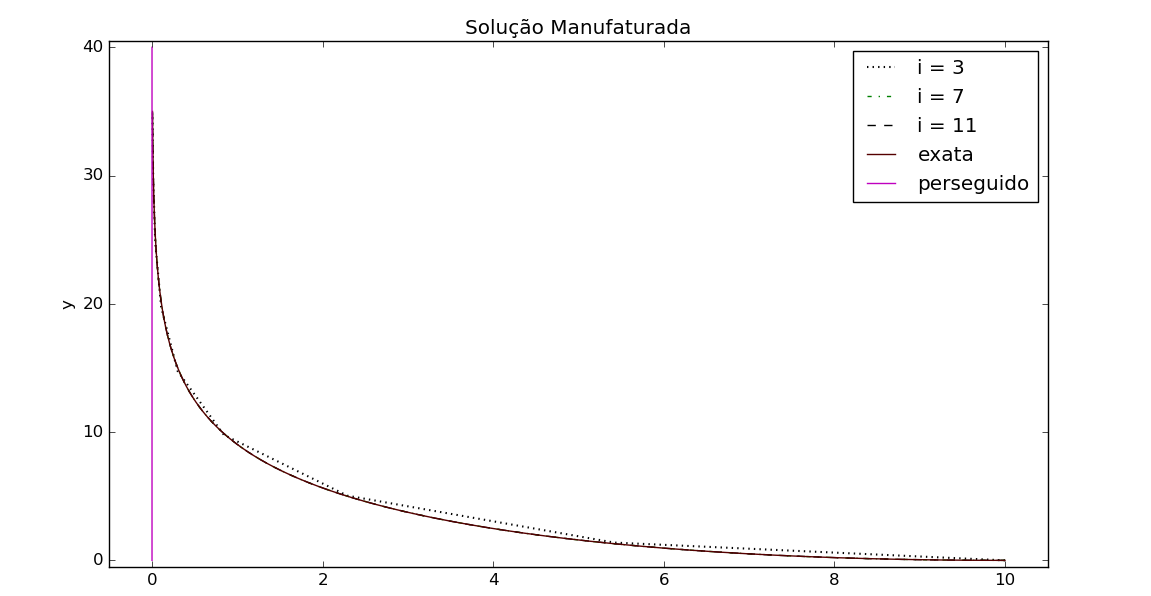
\includegraphics[width=\textwidth]{manufaturada.png}
   \caption{Curvas do perseguido e do perseguidor para o problema teste.}
   \label{fig:manufaturada}
  \end{figure}

  
  Com o método devidamente implementado, podemos analisar a curva descrita pelo perseguidor para os dois casos propostos anteriormente.
 
  O primeiro modelo é quando o alvo percorre uma trajetória elíptica, descrita na seção 3. Neste caso utilizamos os valores para os parâmetros $\alpha = 2$ e $\beta = 1$. Este problema foi resolvido numericamente para o intervalo $[0; 10]$, com $i = 10$. Em um primeiro caso, foi estudado para $\mathbb{U}_{0} = (0, 0)$, ou seja, o perseguidor está inicialmente no centro da elipse. A constante $k$ teve seu valor variado entre 0.5, 1 e 2. A figura \ref{fig:curva-el} apresenta o gráfico de $x(t)$ e de $y(t)$ e a imagem da curva para este modelo.
  
  \begin{figure}[H]
   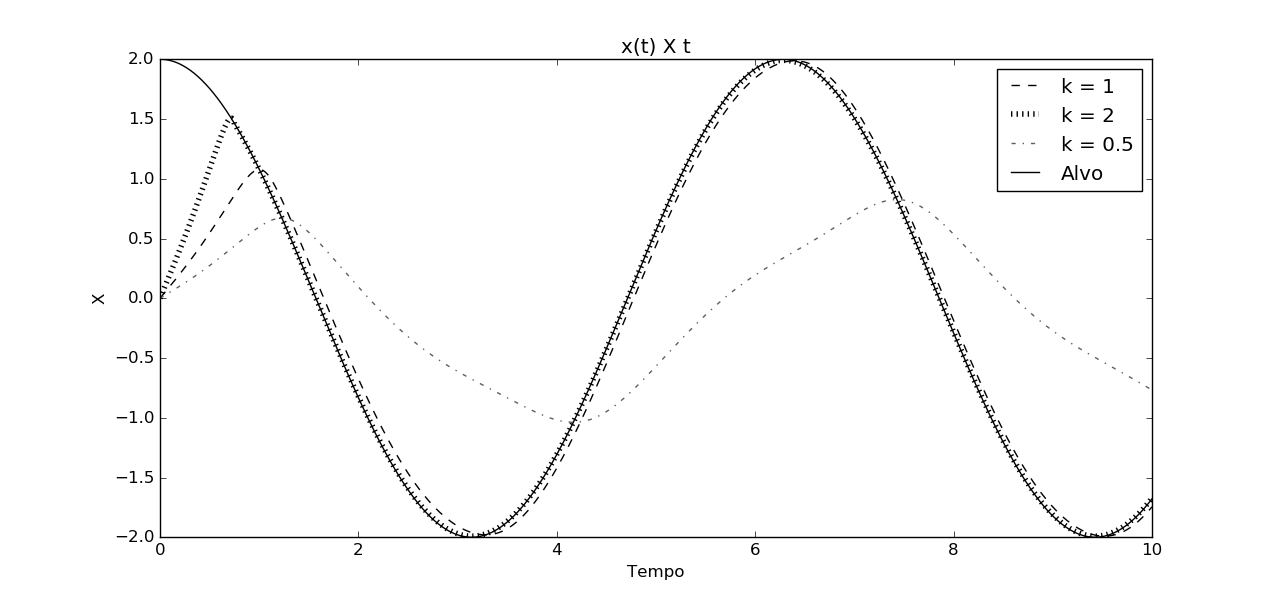
\includegraphics[width=\textwidth]{el-0-X.png}
   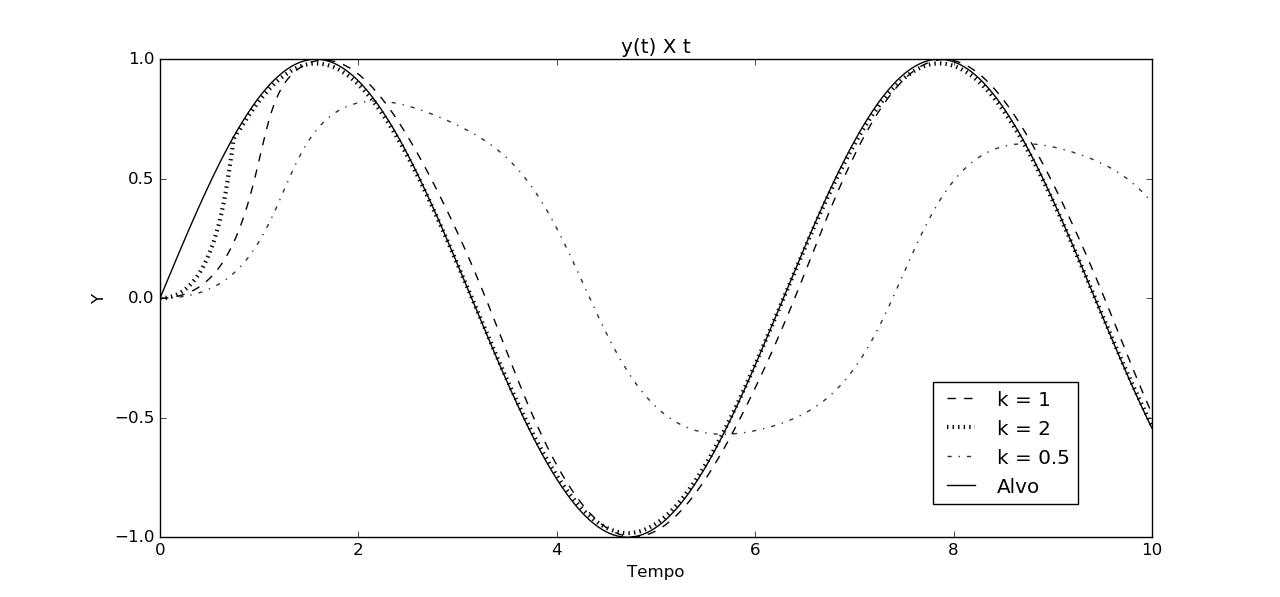
\includegraphics[width=\textwidth]{el-0-Y.png}
   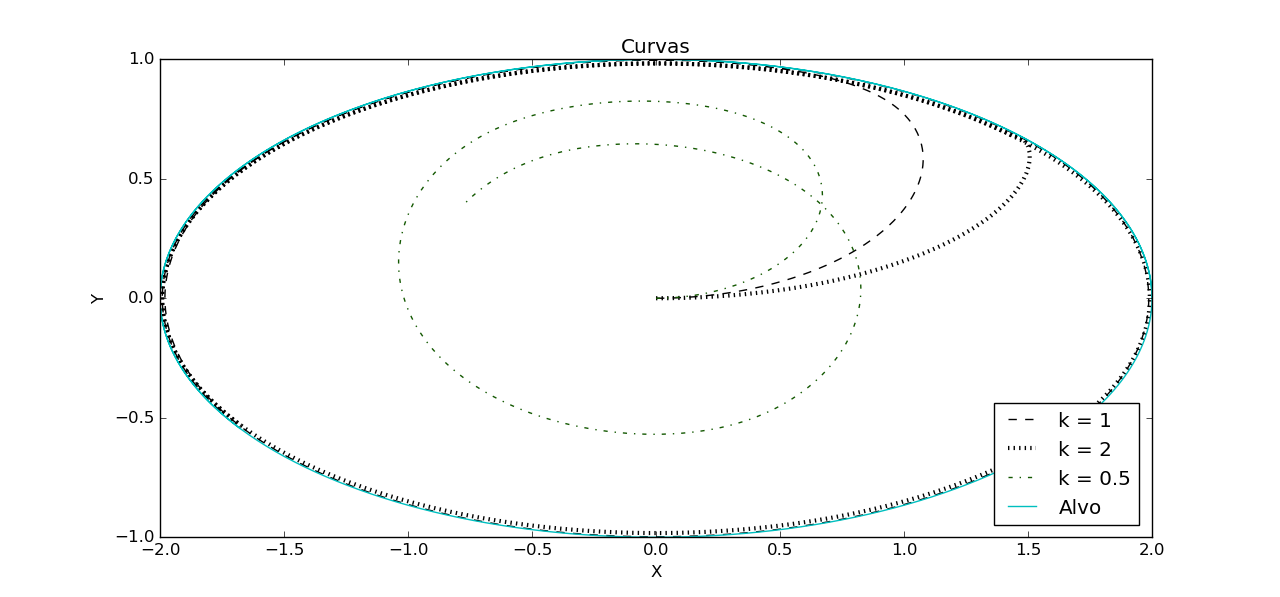
\includegraphics[width=\textwidth]{el-0-XY.png}
   \caption{Curvas de perseguição de um modelo elíptico.}
   \label{fig:curva-el}
  \end{figure}
  
  A partir do gráfico, podemos observar que quando ambos os elementos estão à mesma velocidade, o perseguidor fica muito próximo de sua presa, entretanto, não consegue alcançá-lo. Não obstante, quando ele está com uma velocidade maior, ele consegue capturar a presa. Para a velocidade sendo a metade da velocidade o perseguido, por sua vez, a trajetória descrita pelo perseguidor é parecida com uma elipse, mas com um comprimento menor, i.e., ela é interna à curva descrita pelo alvo.
  
  Para um perseguidor que está inicialmente fora da elipse, o comportamento tende ao mesmo do caso anterior, sendo diferente apenas no inicio. O gráfico para este problema é apresentado na figura \ref{fig:curva-el-1}.
  
   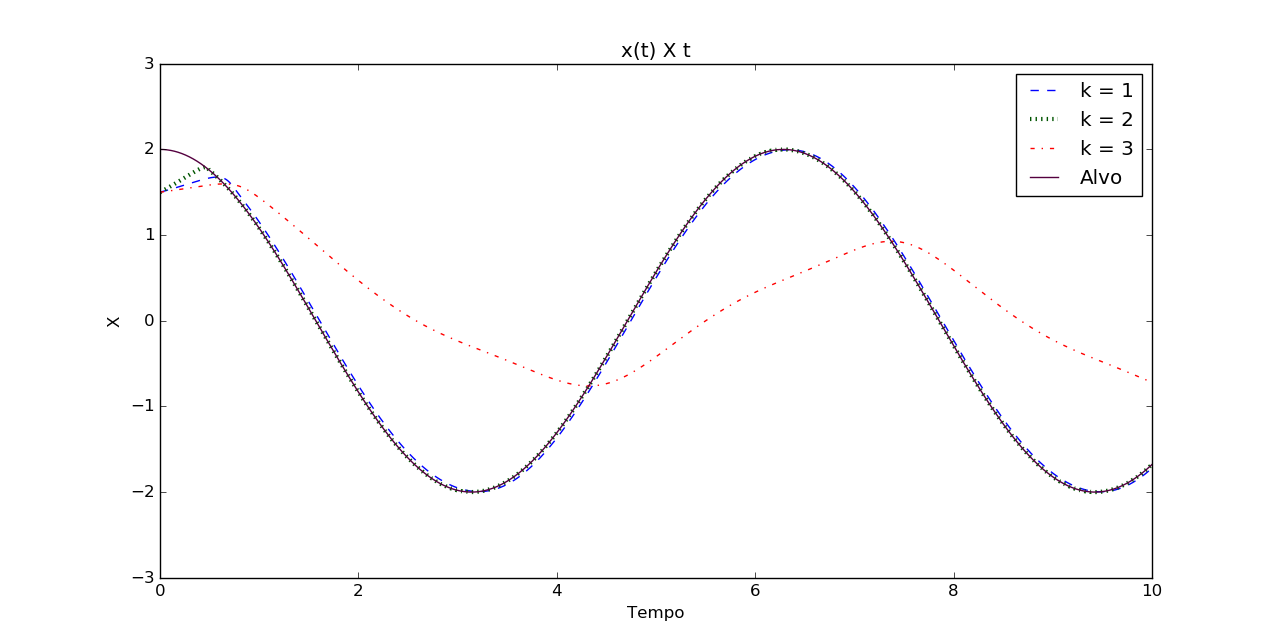
\includegraphics[width=\textwidth]{el-1-X.png}
   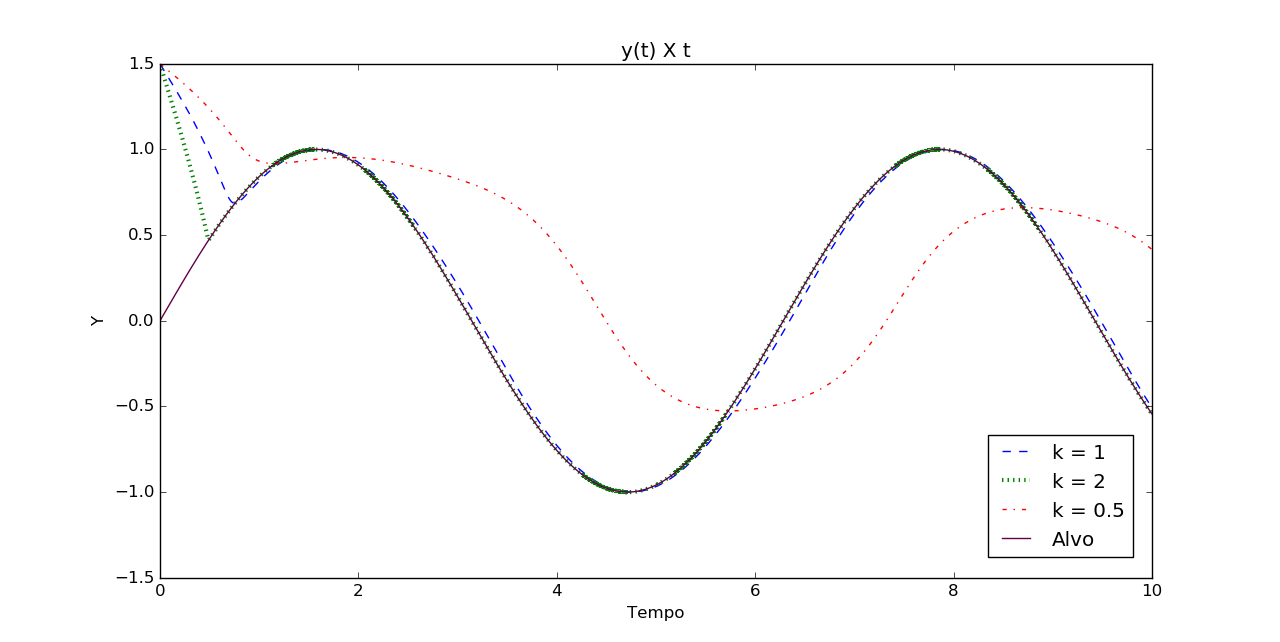
\includegraphics[width=\textwidth]{el-1-Y.png}
   \begin{figure}[H]
   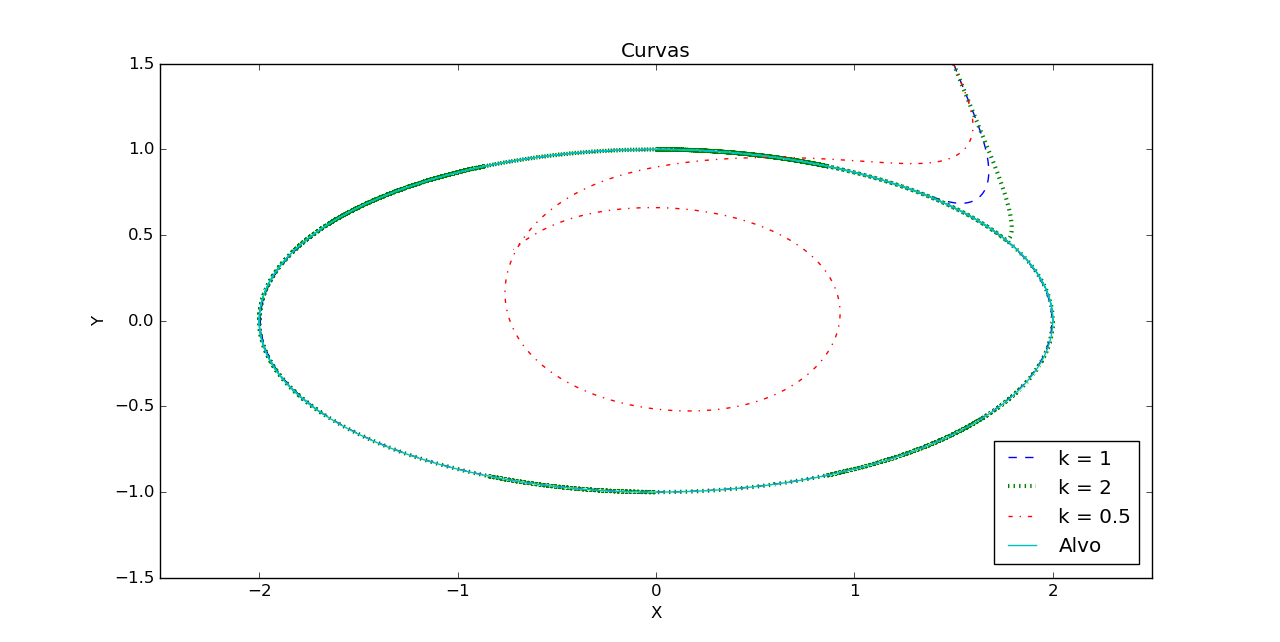
\includegraphics[width=\textwidth]{el-1-XY.png}
   \caption{Curvas de perseguição de um modelo elíptico.}
   \label{fig:curva-el-1}
  \end{figure}
  
  O último modelo a ser estudado é a curva de perseguição para um perseguido que descreve uma trajetória em \emph{zigue-zague}. Neste modelo utilizamos um spline cúbico para interpolar os pontos resultantes da integração e, assim, estudar a curva de maneira contínua. A partir da curva resultante é possível observar que o perseguidor descreve uma trajetória semelhante a uma senóide.
  
  O spline utilizado neste problema realiza a interpolação dos pontos obtidos para a coordenada $y_k$, como função das coordenadas $x_k$. Para a condição de contorno do spline vinculado, foi necessária a obtenção de $\frac{dy(0)}{dx}$ e $\frac{dy(t_n)}{dx}$. Apesar da função $f$ do problema de Cauchy nos retornar os valores de $x'(t)$ e $y'(t)$, podemos facilmente descobrir o desejado pela regra da cadeia:
  \begin{equation}
   \frac{dy}{dx} = \frac{dy}{dt} \frac{dt}{dy}
  \end{equation}
  
  O resultado da solução numérica, juntamente com a interpolação, pode ser vista na figura \ref{fig:curva-zz}.
  
  \begin{figure}[H]
   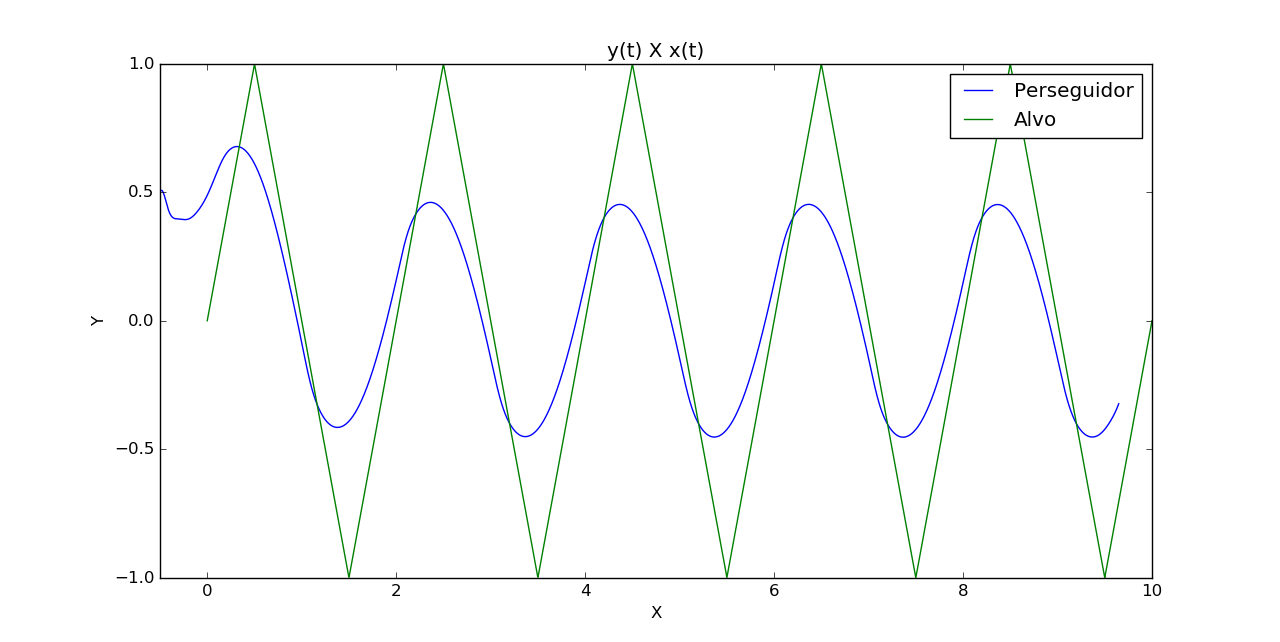
\includegraphics[width=\textwidth]{zz-XY-spline.png}
   \caption{Modelo \emph{ziguezague} com uso da técnica de spline cúbico.}
   \label{fig:curva-zz}
  \end{figure}  
  
  Para essas curvas apresentadas, podemos realizar também uma interpolação pelo método do spline cúbico.
  O algoritmo desse método foi desenvolvido na linguagem Python e foi baseado no algoritmo 3.5 do Numerical Analiysis [4]. 
  Os passos 4, 5, 6 e parte do 7 são responsáveis por resolver o sistema tridiagonal \ref{eq:sistema}.
  \begin{lstlisting}[frame=single]
   def spline(X, A, fpo, fpn):
	n = len(X)-1
	H = np.empty((n + 1))
	Alfa = np.empty((n + 1))
	L = np.empty((n + 1))
	mi = np.empty((n + 1))
	z = np.empty((n + 1))
	C = [0] * (n + 1)
	B = [0] * (n + 1)
	D = [0] * (n + 1)
	
	#### Passo 1 ####

	for i in range(n):
		H[i] = X[i+1] - X[i]
		
	#### Passo 2 ####
		
	Alfa[0] = 3 * (A[1] - A[0])/H[0] - 3 * fpo
	Alfa[n] = 3 * fpn - 3 * (A[n] - A[n-1])/H[n-1]
	
	#### Passo 3 ####

	for j in range(n - 1):
		i = j + 1
		Alfa[i]=(3/H[i]) * (A[i+1]-A[i]) - (3/H[i-1]) * (A[i]-A[i-1])
		
	#### Passo 4 ####
	
	L[0] = 2 * H[0]
	mi[0] = 0.5
	z[0] = Alfa[0] / L[0]

	#### Passo 5 ####
	
	for j in range(n - 1):
		i = j + 1
		L[i] = 2 * (X[i+1] - X[i-1]) - H[i-1]*mi[i-1]
		mi[i] = H[i]/L[i]
		z[i] = (Alfa[i] - H[i-1] * z[i-1]) / L[i]

	#### Passo 6 ####	
	
	L[n] = H[n-1] * (2 - mi[n-1])
	z[n] = (Alfa[n] - H[n-1] * z[n-1]) / L[n]
	C[n] = z[n]
	
	#### Passo 7 ####

	for i in reversed(range(n)):
		C[i] = z[i] - mi[i] * C[i+1]
		B[i] = (A[i+1] - A[i]) / H[i] - H[i] * (C[i+1] + 2 * C[i]) / 3
		D[i] = (C[i+1] - C[i]) / (3 * H[i])

	
  \end{lstlisting}

  \section{Conclusão}
  O presente trabalho nos permitiu desenvolver o processo de obtenção da solução numérica de um problema modelado por um sistema linear de equações diferenciais, mais especificamente, utilizando o método implícito dos trapézios, que também nos permitiu desenvolver a técnica da utilização do método de Newton para a obtenção da raiz de uma função bidimensional.
  
  A partir da verificação do método pela técnica da Solução Manufaturada, foi possível validar o método utilizado, que ainda pode ser utilizado para problemas futuros. Com isso também foi possível verificarmos experimentalmente que o método dos trapézios converge proporcionalmente ao quadrado do passo $h$.
  
  O algoritmo de splines cúbicos implementados também foi validado comparando os coeficientes obtidos com um polinômio de terceiro grau. Seu uso para o problema solucionado numericamente permitiu a obtenção de uma curva contínua através da técnica de interpolação e isso nos proporciona um estudo melhor, caso seja necessário a utilização de um par de pontos que não tenha sido calculado pela integração.
  
  Finalmente, também observou-se neste trabalho as diferentes formas de curvas descrita para um caso de perseguição, mostrando-nos que a perseguição é bem sucedida apenas quando o perseguidor possui uma velocidade maior que seu objetivo. Esta análise de curvas pode ser muito importante para problemas reais, como mencionado na seção \ref{sec:intro}.
  
  \section{Referências bibliográficas}
  \bibliographystyle{unsrt}

  \begin{thebibliography}{9}
    \bibitem{wolfram}
      WEISSTEIN, Eric W.,
      \emph{Pursuit Curve},
      MathWorld--A Wolfram Web Resource,
      Disponível em: http://mathworld.wolfram.com/PursuitCurve.html,
      Acessado 25/03/2016.

    \bibitem{lloyd}
      LLOYD, Michael, Ph.D.,
      \emph{Pursuit Curves},
      Academic Forum 24,
      2006.
      
     \bibitem{humes}
      HUMES, Ana et al. \emph{Noções de Cálculo Numérico}. São Paulo: McGraw-Hill do Brasil, 1984.
     
     \bibitem{burden}
      BURDEN, Richard L.; FAIRES, J. Douglas. \emph{Numerical Analysis}. Boston: Brooks Cole, 2010.  

  \end{thebibliography}
  
  \section{Apêndice}
  \appendix
  \section{Rosas são vermelhas}
  Como citado anteriormente, as curvas de perseguições também geram grande interesse devido aos seus aspectos estéticos, resultando em curvas muitas vezes inusitadas e visualmente agradáveis.
  Motivados por isso, decidimos verificar a curva para uma presa que descreve uma trajetória na forme de rosácea de 9 pétalas e com $k = 0.85$. A figura \ref{fig:rosacea} apresenta o resultado desta curva. O perseguidor, para este caso, descreve uma rosácea de menor comprimento. Realizando o cálculo para diversos valores de $k$ obtemos uma combinação muito interessante de rosáceas.
  
  \begin{figure}[H]
   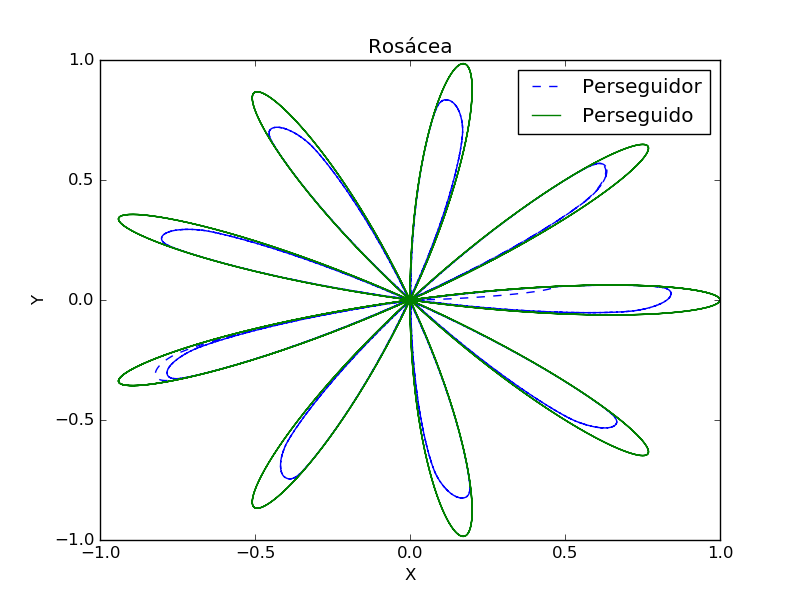
\includegraphics[width=\textwidth]{rosacea.png}
   \caption{Modelo das rosáceas.}
   \label{fig:rosacea}
  \end{figure}
  

\end{document}
